\documentclass[18pt]{article}%
\usepackage{amsfonts}
\usepackage{fancyhdr}
\usepackage{comment}
\usepackage[a4paper, top=2.5cm, bottom=2.5cm, left=2.2cm, right=2.2cm]%
{geometry}
\usepackage{times}
\usepackage{amsmath}
\usepackage{changepage}
\usepackage{amssymb}
\usepackage{hyperref}
\usepackage{graphicx}%
\setcounter{MaxMatrixCols}{30}
\newtheorem{theorem}{Theorem}
\newtheorem{acknowledgement}[theorem]{Acknowledgement}
\newtheorem{algorithm}[theorem]{Algorithm}
\newtheorem{axiom}{Axiom}
\newtheorem{case}[theorem]{Case}
\newtheorem{claim}[theorem]{Claim}
\newtheorem{conclusion}[theorem]{Conclusion}
\newtheorem{condition}[theorem]{Condition}
\newtheorem{conjecture}[theorem]{Conjecture}
\newtheorem{corollary}[theorem]{Corollary}
\newtheorem{criterion}[theorem]{Criterion}
\newtheorem{definition}[theorem]{Definition}
\newtheorem{example}[theorem]{Example}
\newtheorem{exercise}[theorem]{Exercise}
\newtheorem{lemma}[theorem]{Lemma}
\newtheorem{notation}[theorem]{Notation}
\newtheorem{problem}[theorem]{Problem}
\newtheorem{proposition}[theorem]{Proposition}
\newtheorem{remark}[theorem]{Remark}
\newtheorem{solution}[theorem]{Solution}
\newtheorem{summary}[theorem]{Summary}
\newenvironment{proof}[1][Proof]{\textbf{#1.} }{\ \rule{0.5em}{0.5em}}

\newcommand{\Q}{\mathbb{Q}}
\newcommand{\R}{\mathbb{R}}
\newcommand{\C}{\mathbb{C}}
\newcommand{\Z}{\mathbb{Z}}

\begin{document}

\begin{figure}

\includegraphics[height=3cm]{logo.jpg}
\end{figure}
\title{Assignment01}
\author{20146136, Oh Joon-oh}
\date{2018.09.15.}
\maketitle
\section{Introduction}

This is a technical report that describes how to use the git utility.

\section{Git Technique Explanation}
Git utility is widely used by developers. It is because there are several benefits on using the git utility. Main features of git are code sharing, work integration, version control, and open source contribution. At below, this paper explains the way of git usage.

\subsection {Code Sharing}
With the git utility, people can upload their local files to git repository. By this repository, the files can be shared.
In order to upload files, init, add, remote, commit, push commands are needed.


\subsubsection {Init}
Start using the git utility on the local repository.\\
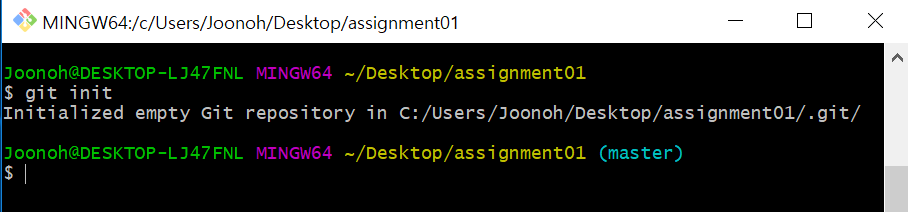
\includegraphics[height=4cm]{init.PNG}

\subsubsection {Add}
Select the files that want to be committed.\\
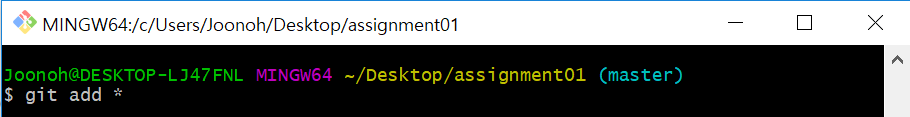
\includegraphics[width=15cm]{add.PNG}

\subsubsection {Commit}
Commit the files to be shared with a comment.\\
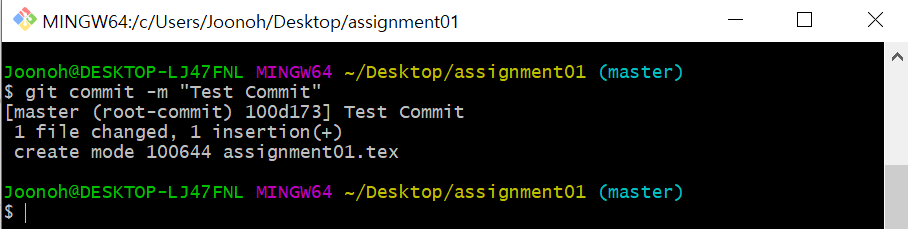
\includegraphics[height=4cm]{commit.PNG}

\subsubsection {Remote}
Define the certain Github repository.\\
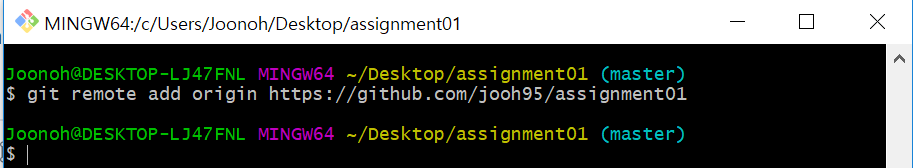
\includegraphics[height=3cm]{remote.PNG}

\subsubsection {Push}
Upload committed files to the certain Github repository.\\
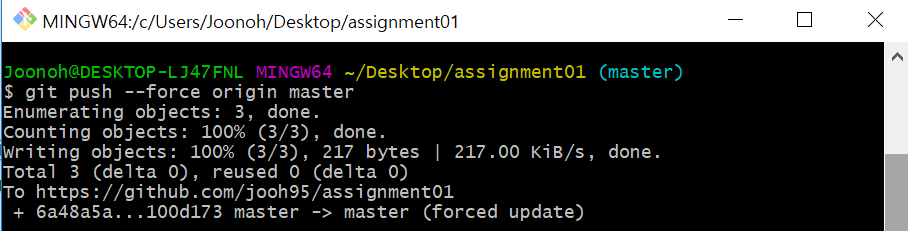
\includegraphics[height=4cm]{push.PNG}


People can view, download, and contribute on this repository. Details about code cloning and contributing will be covered below.\\
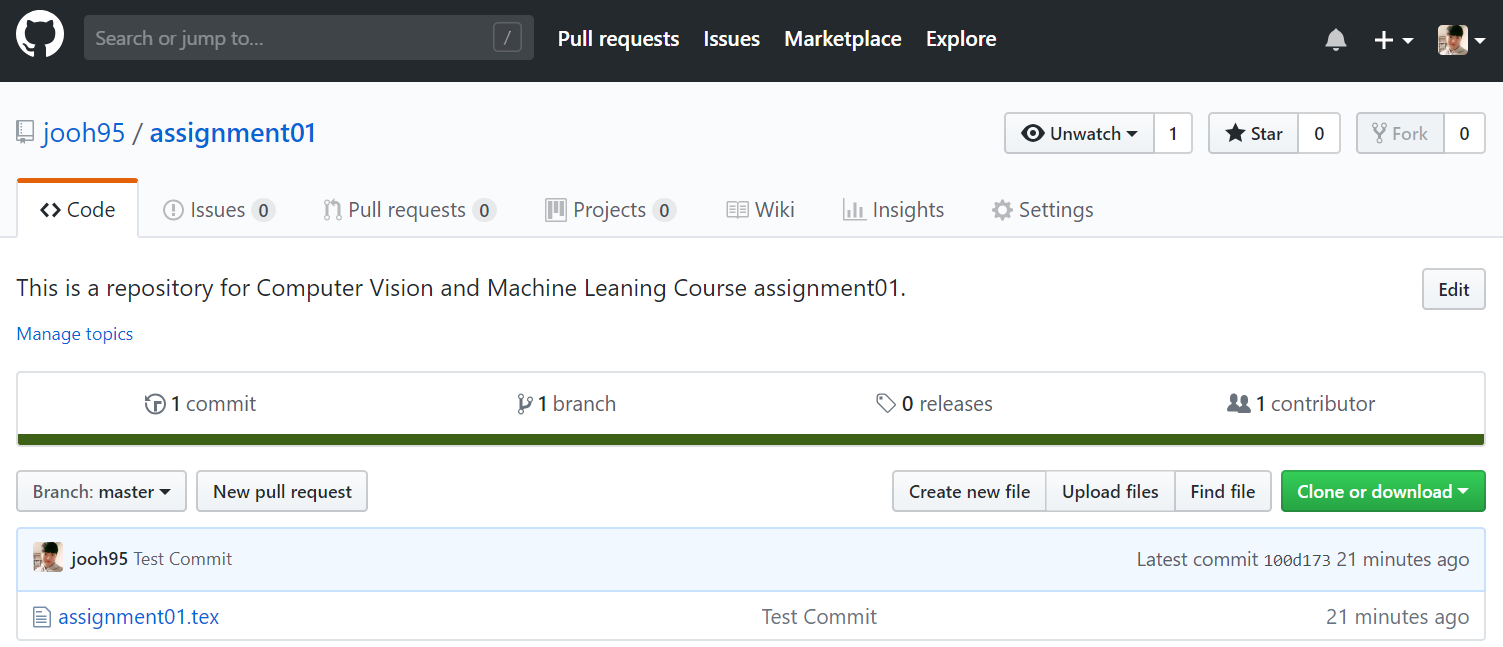
\includegraphics[height=7cm]{upload.PNG}


\subsection {Work Integration}
Git utility is also useful when several people work on the same code or project. Status and pull commands give information about updates on the file so that integration jobs become much easier. Besides, work can be managed separately through the unit called 'branch.'


\subsubsection {Pull}
From the remote Github repository, one can copy others' work to his or her local directory.\\
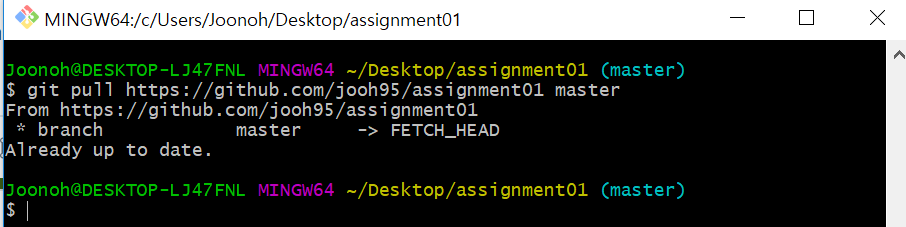
\includegraphics[height=4cm]{pull.PNG}

\subsubsection {Status}
Modifications in the repository are easily checked.\\
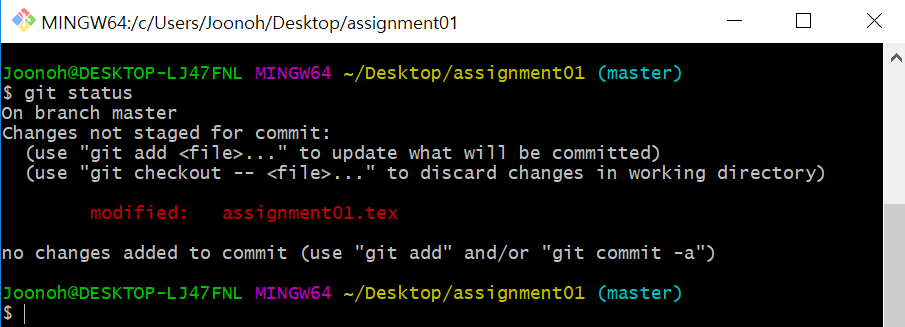
\includegraphics[height=6cm]{status.PNG}

\subsubsection {Branch}
Branch is a unit for managing the repository. There should be many branches in a single project.\\
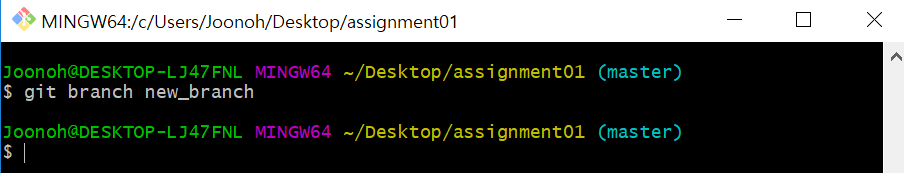
\includegraphics[height=3cm]{branch.PNG}

If there are updates, one can push that modification to the server. Thus, work is always in an integrated status.

 
 \subsection {Version Control}
When working on a project, several version of code or documents are created. Git utility provide roll back function. Moreover, the history of commit is available.

\subsubsection {Reset}
Roll back to the previous commit according to the HEAD pointer with deleting commit history. HEAD is a pointer points the using branch.\\
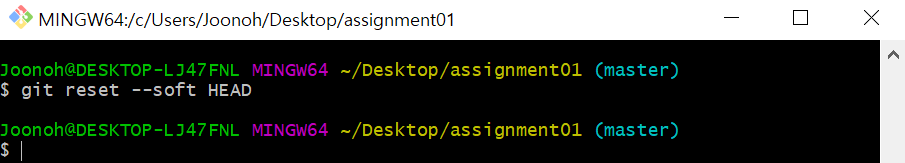
\includegraphics[height=3cm]{reset.PNG}

\subsubsection {Checkout}
Checkout command is similar to the reset command. However, the difference in on checkout command can roll back a certain file.\\
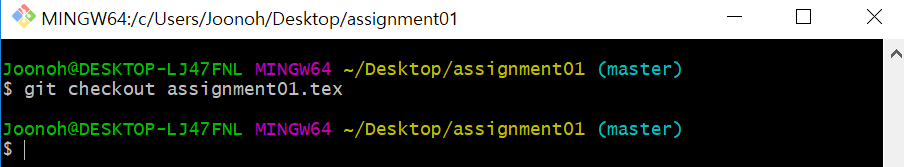
\includegraphics[height=3cm]{checkout.PNG}

\subsubsection {Revert}
Revert is also similar to the reset command, but the commit history is kept.\\
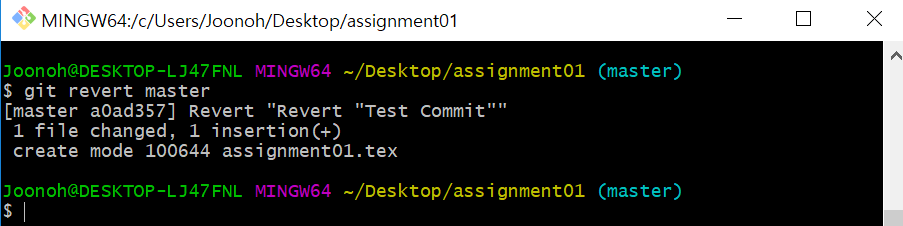
\includegraphics[height=4cm]{revert.PNG}

\subsubsection {Log}
History of users' commit can be tracked by the log command.\\
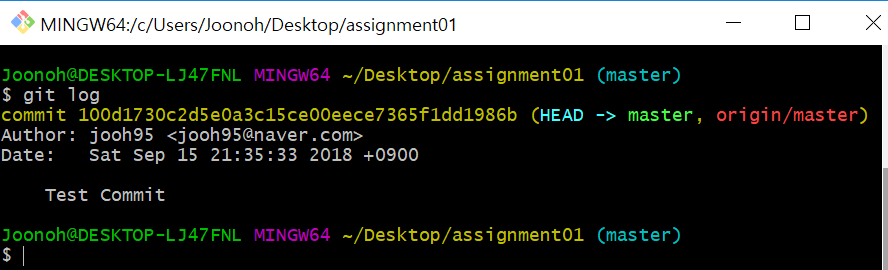
\includegraphics[height=5cm]{log.PNG}

 
 \subsection {Open Source Contribution}
In Github, millions of open source are free to implement. To use those, developers have to clone to their own local repository.

\subsubsection {Clone}
Clone command copies all files from the remote server to the local repository.\\
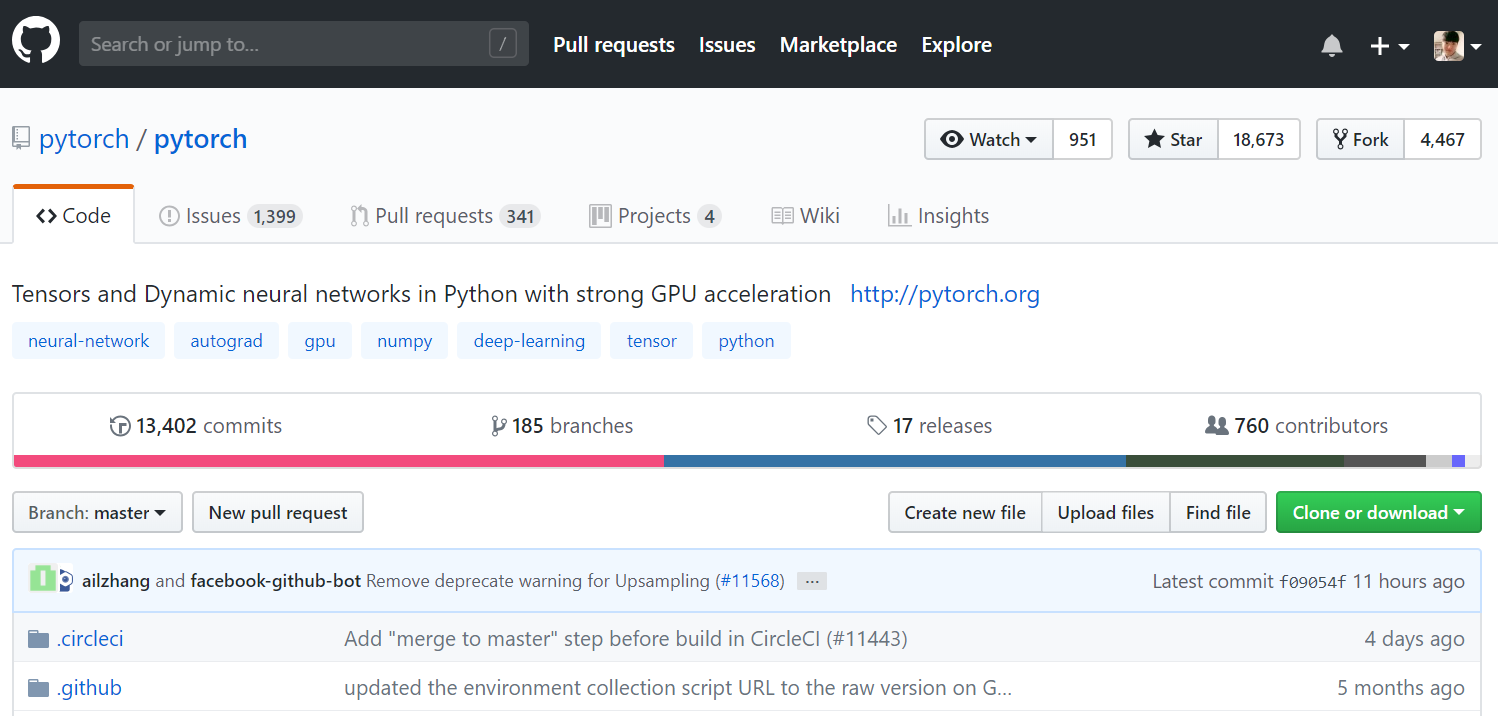
\includegraphics[height=8cm]{pytorch.PNG}
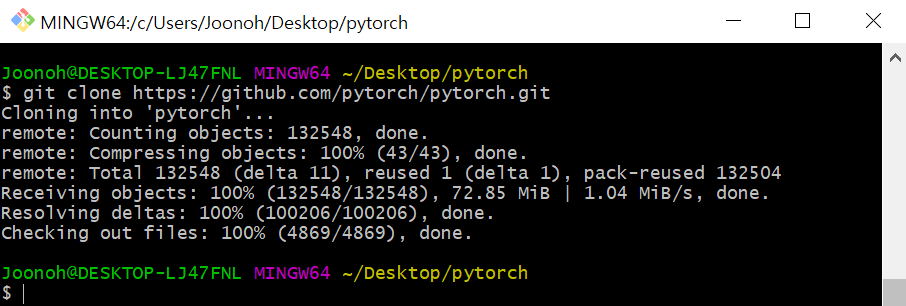
\includegraphics[height=6cm]{clone.PNG}



Through the git, open source developers can improve original code, implement the code on their own projects, ask some questions in issues section, etc. \\



\section{Github Link}

\href{https://github.com/jooh95/assignment01}{https://github.com/jooh95/assignment01}

\end{document}